\chapter{Anhang}
\section{Technischer Aufbau SAP Subscription Billing}
\label{anhang_cf_infrastruktur}
\begin{figure}[h]
	\begin{center}
		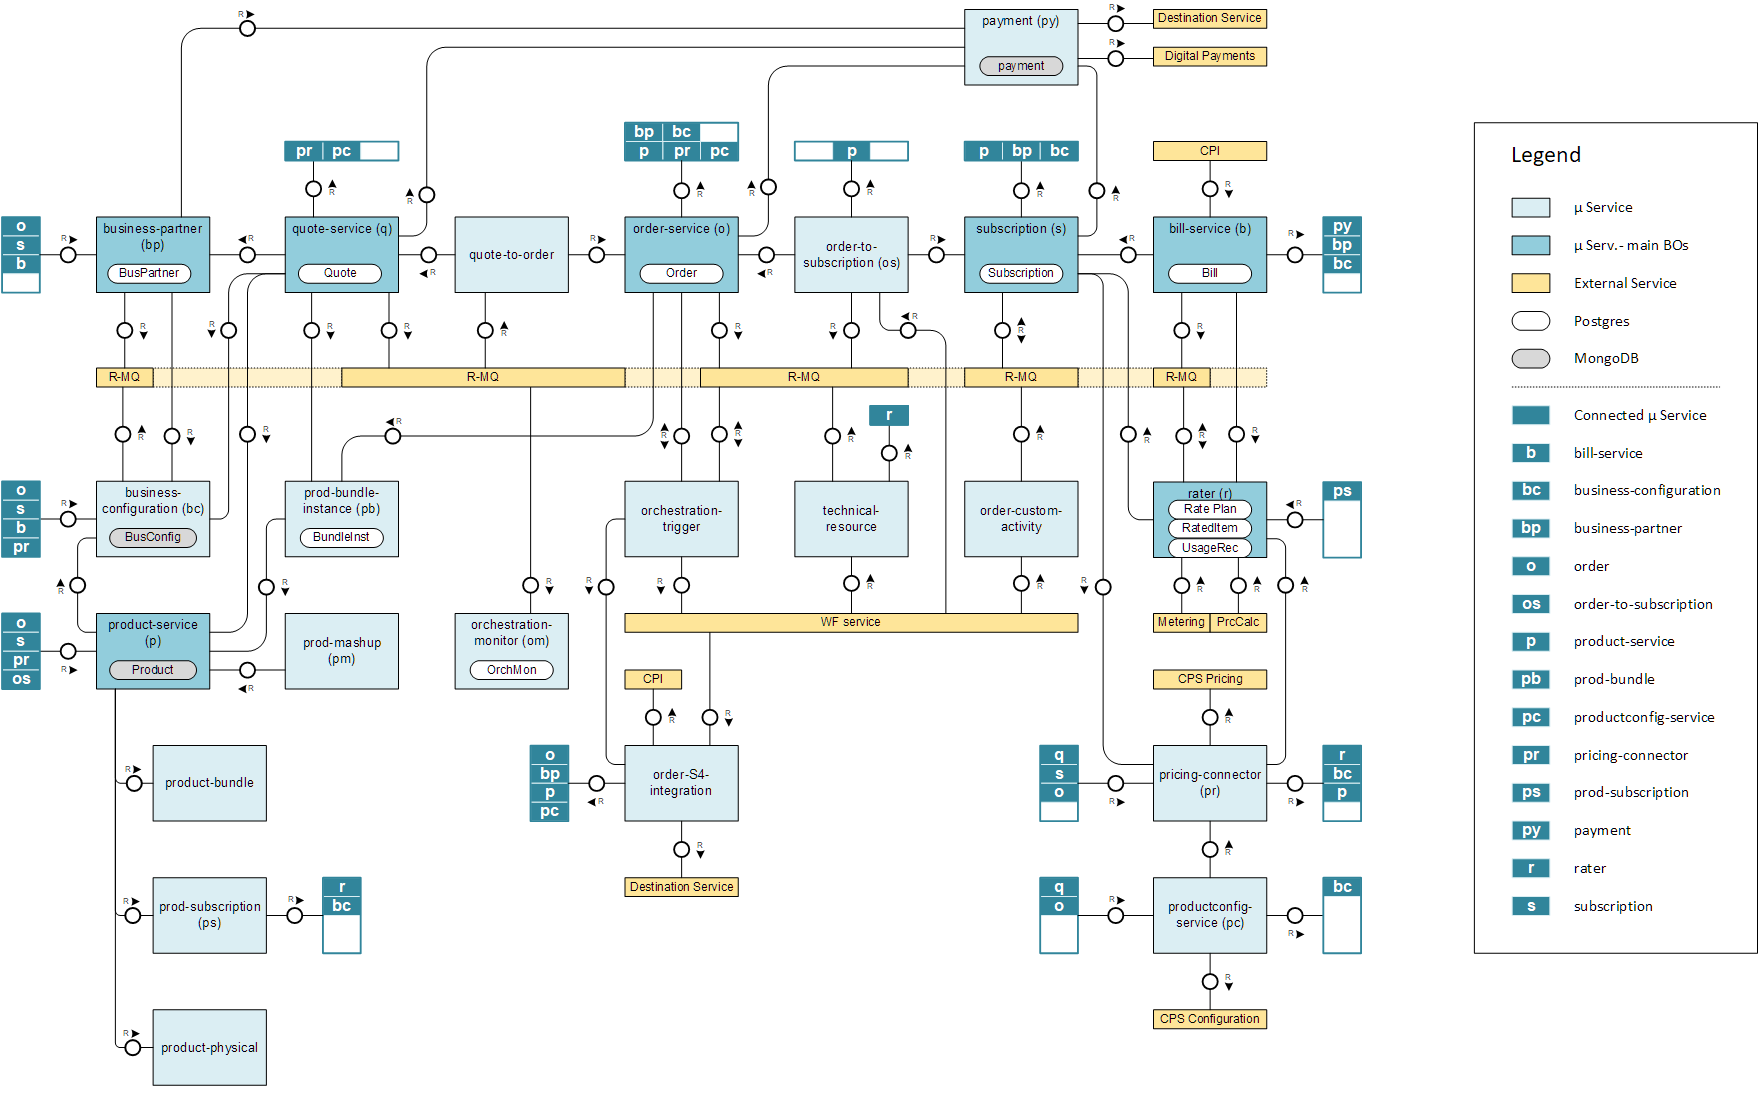
\includegraphics[width=16cm]{img/ssb_microservices.JPG}
		\caption[Technischer Überblick Microservices und Datenbanken der SAP Subschription Billing Softwarelösung]{Technischer Überblick Microservices und Datenbanken der SAP Subschription Billing Softwarelösung\\ (Abbildung stammt aus dem projektinternen Wiki)}
		\label{grafik_ssb_microservices}
	\end{center}
\end{figure}

\newpage
\section{Untersuchung der Performance mittels JMeter}
\subsection{Testsetup für die Messung der Performance}
\label{anhang_performancetests}
Bei der Messung der Performance wurde folgende \ac{HTTPS}-Anfrage an den Endpunkt des Rater-Microservices gesendet. Dabei wurden die jeweiligen extern verfügbaren \acsp{URL} für den Zugriff auf den Rater-Microservice verwendet.\\
\begin{enumerate}
	\item \ac{CF}: \url{https://rater.cfapps.eu10.hana.ondemand.com}
	\item Gardener Kubernetes Cluster: \url{rater.ingress.k8s-sb.subbilling.shoot.canary.k8s-hana.ondemand.com}
	\item Converged Cloud Kubernetes Cluster: \url{https://rater.subscription-billing.c.eu-de-2.cloud.sap}
\end{enumerate}
Es wurde jeweils eine \ac{HTTPS}-POST Anfrage an den folgenden Pfad  mit dem im Quelltext \ref{quellcode_anfrage_performancetests} dargestellten Bodyinhalt gesendet: \textbf{/estimation/public/v1/estimation}\\
Jedoch ist zu beachten, dass hierfür eine erfolgreiche Authentifikation und Autorisierung mittels mehrerer \ac{HTTP}-Header benötigt wird. Es ist zu beachten, dass die angegeben Adressen zwar extern verfügbar sind, jedoch ausschließlich mit einer erfolgreichen Authentifizierung mittels OAuth 2.0 erreichbar sind.\\
Insgesamt wurde jedes Testsetup jeweils mit fünf Testläufen ausgeführt. Dabei betrug das Testintervall der durchgeführten Tests jeweils fünf Minuten pro Testlauf. Dabei wurde jeweils mit 100, 150 und 200 parallelen Threads getestet, welche gleichzeitig zuvor dargestellte \ac{HTTPS}-Anfrage senden.
\newpage
\begin{lstlisting}[language=yaml, caption=Verwendete \acl{HTTPS}-Anfrage für die Messung der Performance, label=quellcode_anfrage_performancetests]
{
	"ratePlans": [
		{
			"id": "${__UUID()}",
			"fixedRates": [
				{
					"id": "${__UUID()}",
					"price": {
						"amount": 5.09,
						"currency": "EUR"
					},
					"metricId": "FIXED_RATE_METRIC_ID",
					"billedInAdvance": false
				}
			],
			"blockRates": [
				{
					"id": "${__UUID()}",
					"pricePerBlock": {
						"amount": 19.81,
						"currency": "EUR"
				},
				"blockSize": 100,
				"metricId": "API_CALL"
				}
			]
		}
	],
	"usageEstimates": [
		{
			"metricId": "API_CALL",
			"quantity": ${__Random(0,1000)}
		}
	]
}
\end{lstlisting}
\newpage
\subsection{Ergebnisse der Performancetests der beiden Plattformen}
\label{section_performance_test}
\subsubsection{Cloud Foundry Umgebung in Frankfurt}
\label{section_performance_test_cf}
\begin{figure}[h]
	\begin{center}
		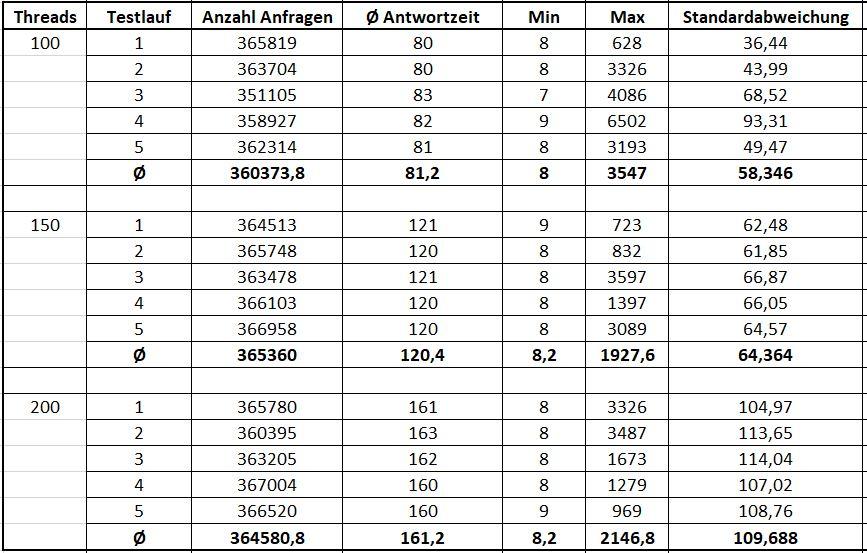
\includegraphics[width=16cm]{img/performance_cf_1.JPG}
		\caption[Performancetests: Cloud Foundry Teil 1]{Ergebnisse Performancetests: Cloud Foundry Teil 1}
		\label{performance_cf_1}
	\end{center}
\end{figure}
\newpage
\begin{figure}[h]
	\begin{center}
		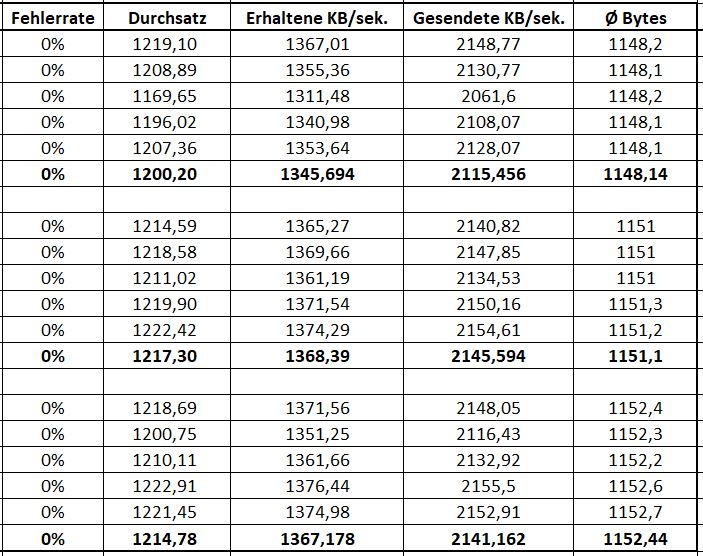
\includegraphics[width=16cm]{img/performance_cf_2.JPG}
		\caption[Performancetests: Cloud Foundry Teil 2]{Ergebnisse Performancetests: Cloud Foundry Teil 2}
		\label{performance_cf_2}
	\end{center}
\end{figure}
\newpage
\subsubsection{Gardener Kubernetes Cluster in Belgien}
\label{section_performance_k8s_gardener}
\begin{figure}[h]
	\begin{center}
		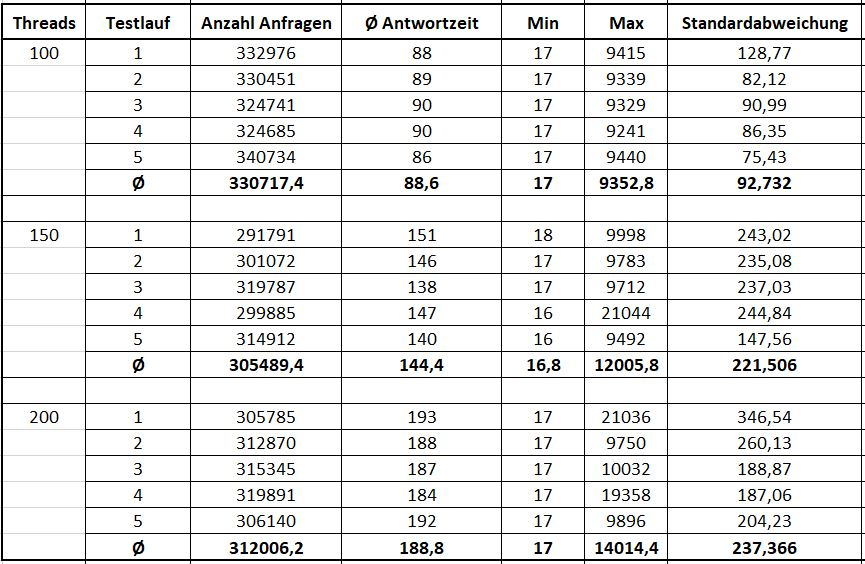
\includegraphics[width=16cm]{img/performance_k8s_1.JPG}
		\caption[Performancetests: Gardener Kubernetes Cluster Teil 1]{Ergebnisse Performancetests: Gardener Kubernetes Cluster Teil 1}
		\label{performance_k8s_1}
	\end{center}
\end{figure}
\newpage
\begin{figure}[h]
	\begin{center}
		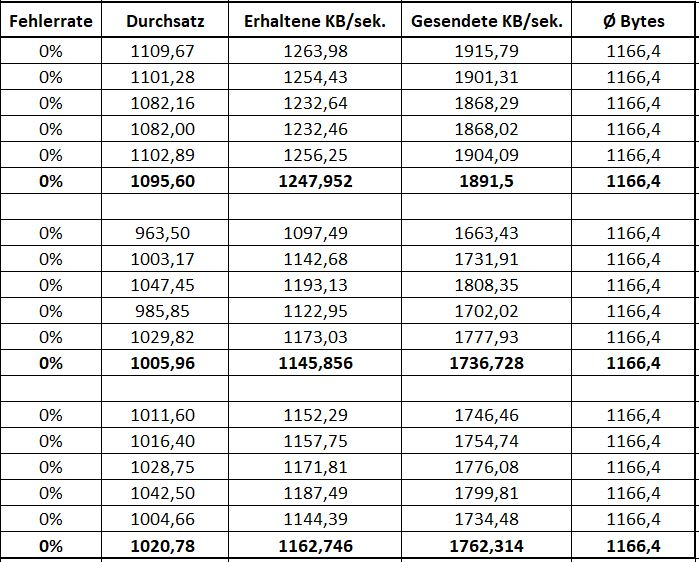
\includegraphics[width=16cm]{img/performance_k8s_2.JPG}
		\caption[Performancetests: Gardener Kubernetes Cluster Teil 2]{Ergebnisse Performancetests: Gardener Kubernetes Cluster Teil 2}
		\label{performance_k8s_2}
	\end{center}
\end{figure}
\newpage
\subsubsection{Converged Cloud Kubernetes Cluster in Frankfurt}
\label{section_performance_k8s_con_cloud}
\begin{figure}[h]
	\begin{center}
		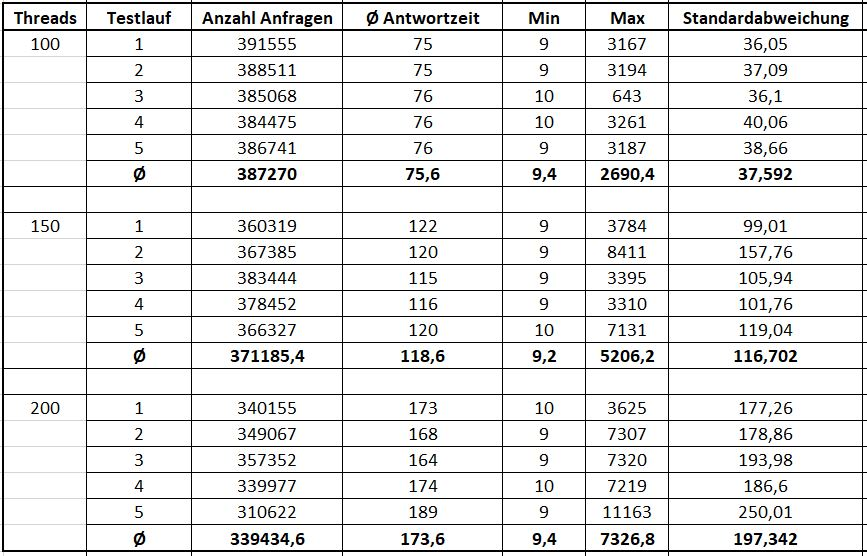
\includegraphics[width=16cm]{img/performance_con_cloud_1.JPG}
		\caption[Performancetests: Converged Cloud Kubernetes Cluster Teil 1]{Ergebnisse Performancetests: Converged Cloud Kubernetes Cluster Teil 1}
		\label{performance_con_cloud_1}
	\end{center}
\end{figure}
\newpage
\begin{figure}[h]
	\begin{center}
		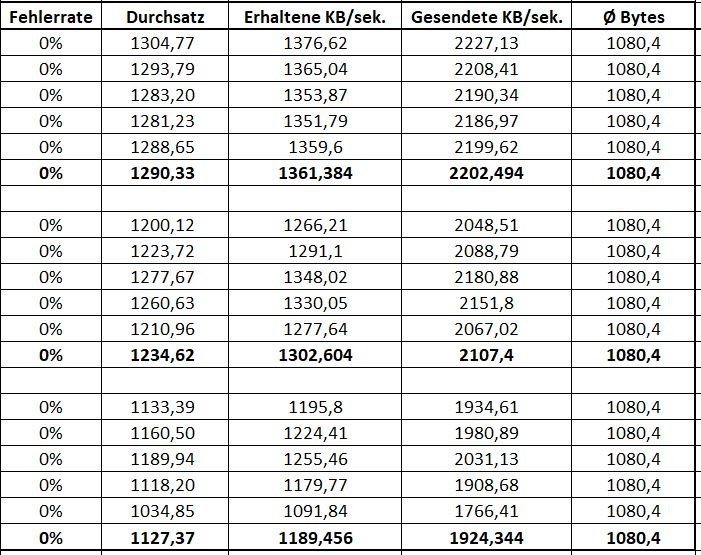
\includegraphics[width=16cm]{img/performance_con_cloud_2.JPG}
		\caption[Performancetests: Converged Cloud Kubernetes Cluster Teil 2]{Ergebnisse Performancetests: Converged Cloud Kubernetes Cluster Teil 2}
		\label{performance_con_cloud_2}
	\end{center}
\end{figure}

\newpage

\section{Beispielhafte Manifestdateien und Quellcode}
\subsection{Bereitstellung der Microservices}
\begin{lstlisting}[language=yaml, caption=Dockerfile des Rater-Microservices, label=quellcode_bereitstellung_microservices]
FROM openjdk: 8-jdk-alpine
ADD /target/rating-rater-0.48.0-SNAPSHOT-exec.jar app.jar
ENTRYPOINT ["java","-Djava.security.egd=file:/dev/./urandom","-jar","/app.jar"]
\end{lstlisting}
Für die Bereistellung der Microservices wird das Open Source Java Development Kit \textbf{OpenJDK} verwendet.\footnote{Offizielles OpenJDK Docker-Image: \url{https://hub.docker.com/_/openjdk}}
Zudem wird die ausführbare \textbf{app.jar}-Datei in den Container kopiert. Diese wird nach erfolgreichem Start des Containers von der lokalen Java Runtime ausgeführt. Das hierfür verwendete Kommando ist der dritten Zeile des zuvor dargestellten Dockerfiles zu entnehmen.\\
\\
Aus den folgenden Quelltexten sind beispielhafte Manifestdateien, welche für die Bereitstellung der Microservices implementiert worden sind. Diese können theoretisch für jedes beliebiges Kubernetes Cluster wiederverwendet werden. Allerdings wird hierfür der in den Manifestdateien definierte Namespace \textbf{dev} sowie die Secrets und die Config Maps benötigt. Aus Sicherheitsgründen kann das Secret für den Zugriff auf die SAP eigene Docker Registry nicht innerhalb der vorliegenden Thesis inkludiert werden.
\\
\lstinputlisting[language=yaml, caption=Beispielhafte Manifestdatei für das Stateful Set des Rater-Microservice, label=quellcode_statefulset_rater]{quellcode/rater.statefulset.yaml}
\newpage
\lstinputlisting[language=yaml, caption=Beispielhafte Manifestdatei für den Horizontal Pod Autoscaler des Rater-Microservices, label=quellcode_hpa_rater]{quellcode/rater.hpa.yaml}
\lstinputlisting[language=yaml, caption=Beispielhafte Manifestdatei für die Config Map des Rater-Microservices, label=quellcode_cm_rater]{quellcode/rater.configmap.yaml}
\newpage
\lstinputlisting[language=yaml, caption=Beispielhafte Manifestdatei für das Stateful Set der MongoDB-Instanz für den Business-Config-Microservice, label=quellcode_statefulset_mongodb]{quellcode/mongodb.statefulset.yaml}
\newpage
\lstinputlisting[language=yaml, caption=Beispielhafte Manifestdatei der \acl{GCP} spezifischen Storage Class zur persistenten Speicherung der Daten, label=quellcode_storageclass_gcp]{quellcode/mongodb.statefulset.yaml}
\newpage
\subsection{Verschiedene Landschaften}
\label{quellcode_verschiedene_landschaften}
\lstinputlisting[language=yaml, caption=Beispielhafte Manifestdatei für den Namespace dev, label=quellcode_namespaces]{quellcode/namespaces.yaml}
\lstinputlisting[language=yaml, caption=Beispielhafte Manifestdatei für den Ingress Service, label=quellcode_ingress_service]{quellcode/global.ingress.yaml}
\newpage
\lstinputlisting[language=yaml, caption=Beispielhafte Manifestdatei für das Default Gateway von Istio, label=quellcode_default_gateway]{quellcode/global.istio.gateway.yaml}
\lstinputlisting[language=yaml, caption=Beispielhafte Manifestdatei für die Destination Rule des Rater-Microservices, label=quellcode_routing_dr]{quellcode/rater.destinationrule.yaml}
\newpage
\lstinputlisting[language=yaml, caption=Beispielhafte Manifestdatei für den für das Routing der externen Anfragen verwendeten Virtual Service, label=quellcode_routing_vs]{quellcode/routing.virtualservice.ext.yaml}
\lstinputlisting[language=yaml, caption=Beispielhafte Manifestdatei für den Service der externen Anfragen des Rater-Microservices, label=quellcode_ext_service_rater]{quellcode/rater.service.ext.yaml}
\newpage
\lstinputlisting[language=yaml, caption=Network Policy für den Business-Config-Microservice, label=quellcode_business-config_np]{quellcode/business-config.networkpolicy.yaml}
\newpage
\subsection{Integration in die \acs{CI}/\acs{CD}-Pipeline}
\lstinputlisting[language=yaml, caption=Manifestdatei für das Skaffold Tool, label=quellcode_skaffold_rater]{quellcode/skaffold.yaml}
\newpage
\begin{lstlisting}[language=yaml, caption=Erweiterung Jenkinsfile um K8s Deployment Stage, label=quellcode_rater_jenkinsfile]
	@Library('ngom-modules')
	import com.sap.billcrowd.jenkins.execution.*
	import com.sap.billcrowd.jenkins.model.*
	
	node {
		try {
			k8sDeployment()
		} 
		catch (Exception e) {
			currentBuild.result = 'FAILURE'
			new BuildStatusEmail(this).sendEmail(e)
			throw e
		} 
		finally {
			deleteDir()
		}
	
	}
	
	def k8sDeployment() {
		try {
			PipelineUtil.sbDockerBuildTools(this, {
				stage("K8s Deployment") {
					container("skaffold") {
						unstash "dir"
						sh "skaffold run"
					}
				}
			})
		} catch (Exception e) {}
	}
\end{lstlisting}
\newpage
\subsection{Service-to-Service Kommunikation}
\label{anhang_s2s_kommunikation}
\lstinputlisting[language=yaml, caption=Beispielhafte Manifestdatei für den Service des Rater-Microservices, label=quellcode_rater_service]{quellcode/rater.service.yaml}
\newpage
\lstinputlisting[language=yaml, caption=Beispielhafte Manifestdatei für den Virtual Service des Rater-Microservices, label=quellcode_rater_vs]{quellcode/rater.virtualservice.yaml}
\lstinputlisting[language=yaml, caption=Globale \acl{mTLS}-Policy für den Istio Service Mesh, label=quellcode_globale_mtls_policy]{quellcode/global.mtlspolicy.yaml}

\clearpage

\section{Monitoring und Logging des Prototyps}
\begin{figure}[h]
	\begin{center}
		\includegraphics[width=16cm]{img/kibana_logs.PNG}
		\caption[Überblick Kibana Dashboard für Logs von Business-Config Microservice]{Überblick Kibana Dashboard für Logs von Business-Config Microservice}
		\label{anhang_grafik_kibana_dashboard}
	\end{center}
\end{figure}
\begin{figure}[h]
\begin{center}
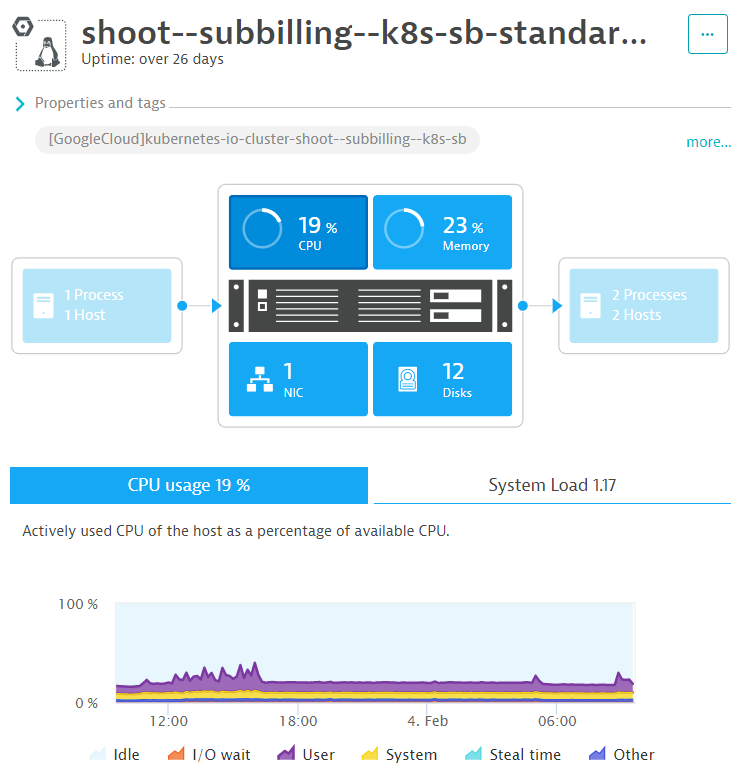
\includegraphics[width=16cm]{img/Dynatrace_Node_Monitoring.PNG}
\caption[Übersicht Dynatrace Dashboard für Monitoring einer Worker Node]{Übersicht Dynatrace Dashboard für Monitoring einer Worker Node}
\label{anhang_grafik_dynatrace_dashboard}
\end{center}
\end{figure}

\clearpage

\section{Zusätzliche Funktionalitäten des Kubernetes Protoyps}
\subsection{Kiali Tool für die Steuerung der Netzwerkkommunikation}
\begin{figure}[h]
	\begin{center}
		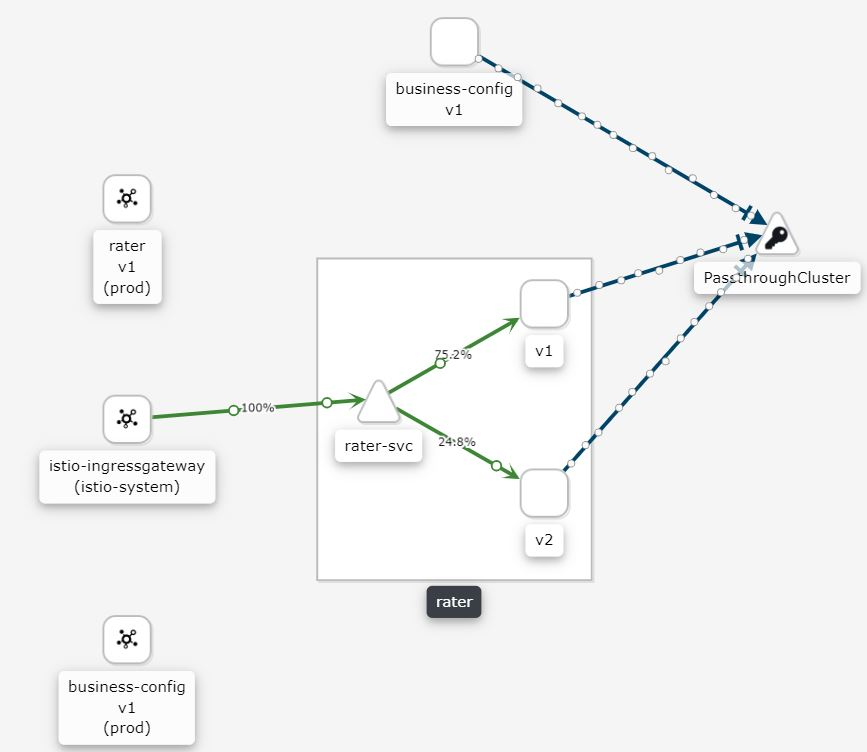
\includegraphics[width=16cm]{img/kiali_dashboard.JPG}
		\caption[Übersicht Routing externer Anfragen mittels Kiali Graphenansicht]{Übersicht Routing externer Anfragen mittels Kiali Graphenansicht}
		\label{anhang_kiali_dashboard}
	\end{center}
\end{figure}
\newpage
\begin{figure}[h]
	\begin{center}
		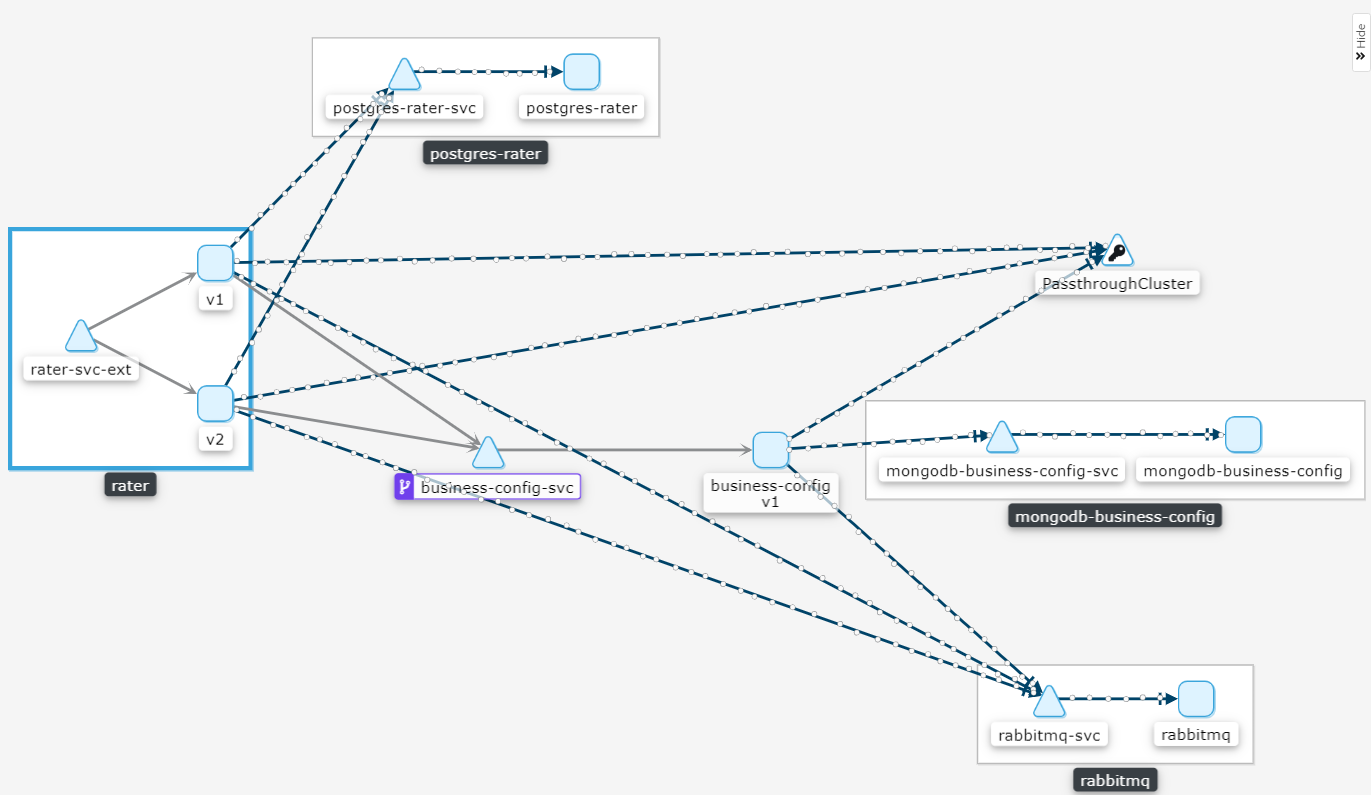
\includegraphics[width=16cm]{img/kiali_dashboard_2.PNG}
		\caption[Übersicht Netzwerkkommunikation mittels Kiali Graphenansicht]{Übersicht Netzwerkkommunikation mittels Kiali Graphenansicht}
		\label{anhang_kiali_dashboard}
	\end{center}
\end{figure}

\newpage

\subsection{Konzept zur Bereitstellung aller Microservices}
\label{anhang_umsetzung_komplettes_Deployment}
Wie in Kapitel \ref{ausblick} erwähnt wurde ein über den Rahmen der vorliegenden Thesis hinausgehendes Konzept für die automatische Bereitstellung aller Microservices der SAP Subscription Billing Lösung entwickelt und prototypisch umgesetzt.\\
Dabei sollte mit Hilfe eines Groovy Skriptes die vollständige Bereitstellung aller Microservices, welche in einem Vektor hinterlegt sind, in einem extra dafür neu angelegten Namespace auf dem Kubernetes Cluster bereitgestellt werden. Dabei ist zu erwähnen, dass auch der Namespace und alle weiteren benötigten Kubernetes-Objekte innerhalb des Prozesses automatisch neu erstellt werden.\\
Ziel des Konzeptes und des Prototyps ist die exemplarische Bereitstellung der Microservices in der im Vektor hinterlegten Version. Dadurch soll jede in der Vergangenheit vorgekommene Konstellation an Microservices in der richtigen Version nachgestellt werden können.\\
Die generellen Schritte des Skriptes sind der Abbildung \ref{anhang_k8s_vector_deployments} zu entnehmen.
\begin{figure}[h]
	\begin{center}
		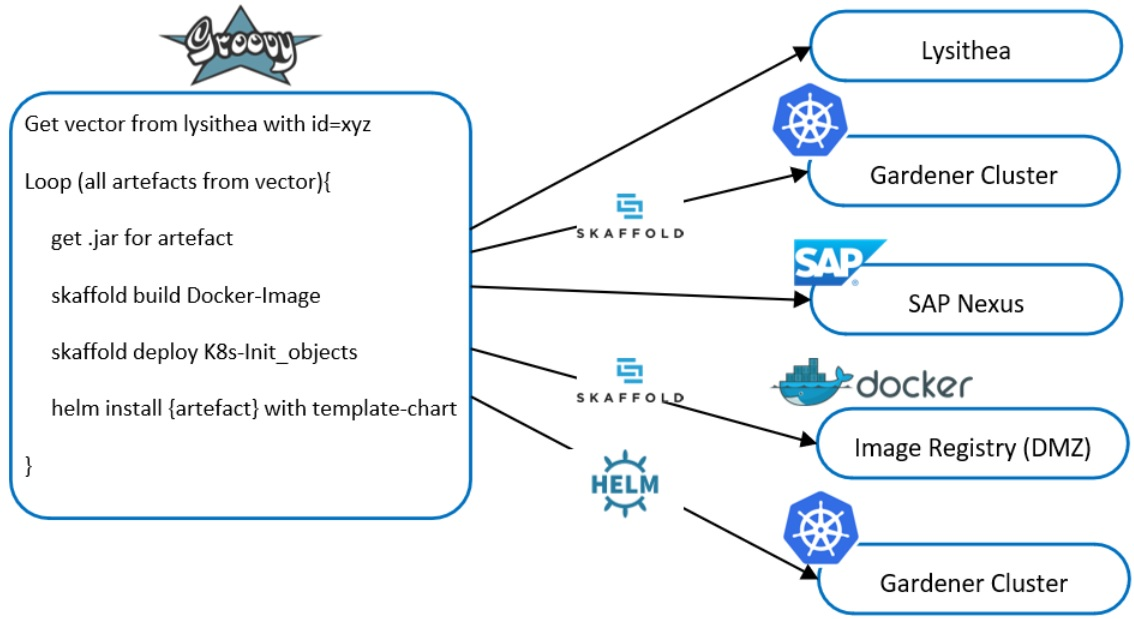
\includegraphics[width=16cm]{img/k8s_vector_deployment.JPG}
		\caption[Übersicht Funktionsweise automatisierten Bereitstellung aller Microservices]{Übersicht Funktionsweise automatisierten Bereitstellung aller Microservices}
		\label{anhang_k8s_vector_deployments}
	\end{center}
\end{figure}
Dabei wird innerhalb des Skriptes die aktuell noch manuell eingegebene ID des Vektors verwendet, um alle Informationen des Vektors und dessen Inhalt aus dem Lysithea-Service anfragen zu können.\\
Anschließend erfolgt mit Hilfe des Skaffold Tools die initiale Installation des Kubernetes Namespaces und der Secrets.\\
Danach beginnt eine Schleife, welche über alle Microservice-Artefakte des Vektors looped. 
Dabei wird für jedes Artefakt die folgenden Schritte durchgeführt:
\begin{enumerate}
	\item Herunterladen des Microservice Artefaktes aus dem SAP Nexus Repository
	\item Bauen des Docker-Images mit Hilfe der lokalen Docker Runtime
	\item Kennzeichnen des Docker-Images mittels der Version des Artefaktes
	\item Hochladen des Docker-Images auf die extern verfügbare Docker Registry von SAP
	\item Automatische Bereitstellung des Microservices mit Hilfe der Helm \ac{CLI} und der des eigens dafür erstellten Helm Charts auf das Kubernetes Cluster
\end{enumerate}
Hierbei ist zu erwähnen, dass mit Hilfe des eigens erstellten Helm Charts generelle Template Manifestdateien für alle benötigten \ac{API}-Objekte von Kubernetes und Istio definiert wurden.\\
Eine beispielhaftes Helm Template, welches für die Definition eines Stateful Sets zur Bereitstellung des eigentlichen Microservices verwendet wird, ist aus dem Quelltext \ref{quellcode_helm_template_ss} zu entnehmen. Ein weiteres Helm Template für die Bereitstellung der Virtual Services je Microservice ist in dem Quelltext \ref{quellcode_helm_template_vs} zu finden.
\\
\lstinputlisting[language=yaml, caption=Beispielhafte Manifestdatei des Helm Templates für das Stateful des Rater-Microservices, label=quellcode_helm_template_ss]{quellcode/microservice.statefulset.yaml}
\newpage
\lstinputlisting[language=yaml, caption=Beispielhafte Manifestdatei des Helm Templates für die Virtual Services der  Microservices, label=quellcode_helm_template_vs]{quellcode/microservice.virtualservice.yaml}
